\chapter{A játék működése}

\thispagestyle{fancy}
\pagestyle{fancy}
\section{Játék ismertetése}

A játék melyet lefejlesztettem, a közismert memória játék.

A játékban az asztalon meghatározott számú kártya pár található, képpel lefelé fordítva, ahogyan az a \ref{img:asztal}. ábrán is látható.
\begin{figure}[h]
    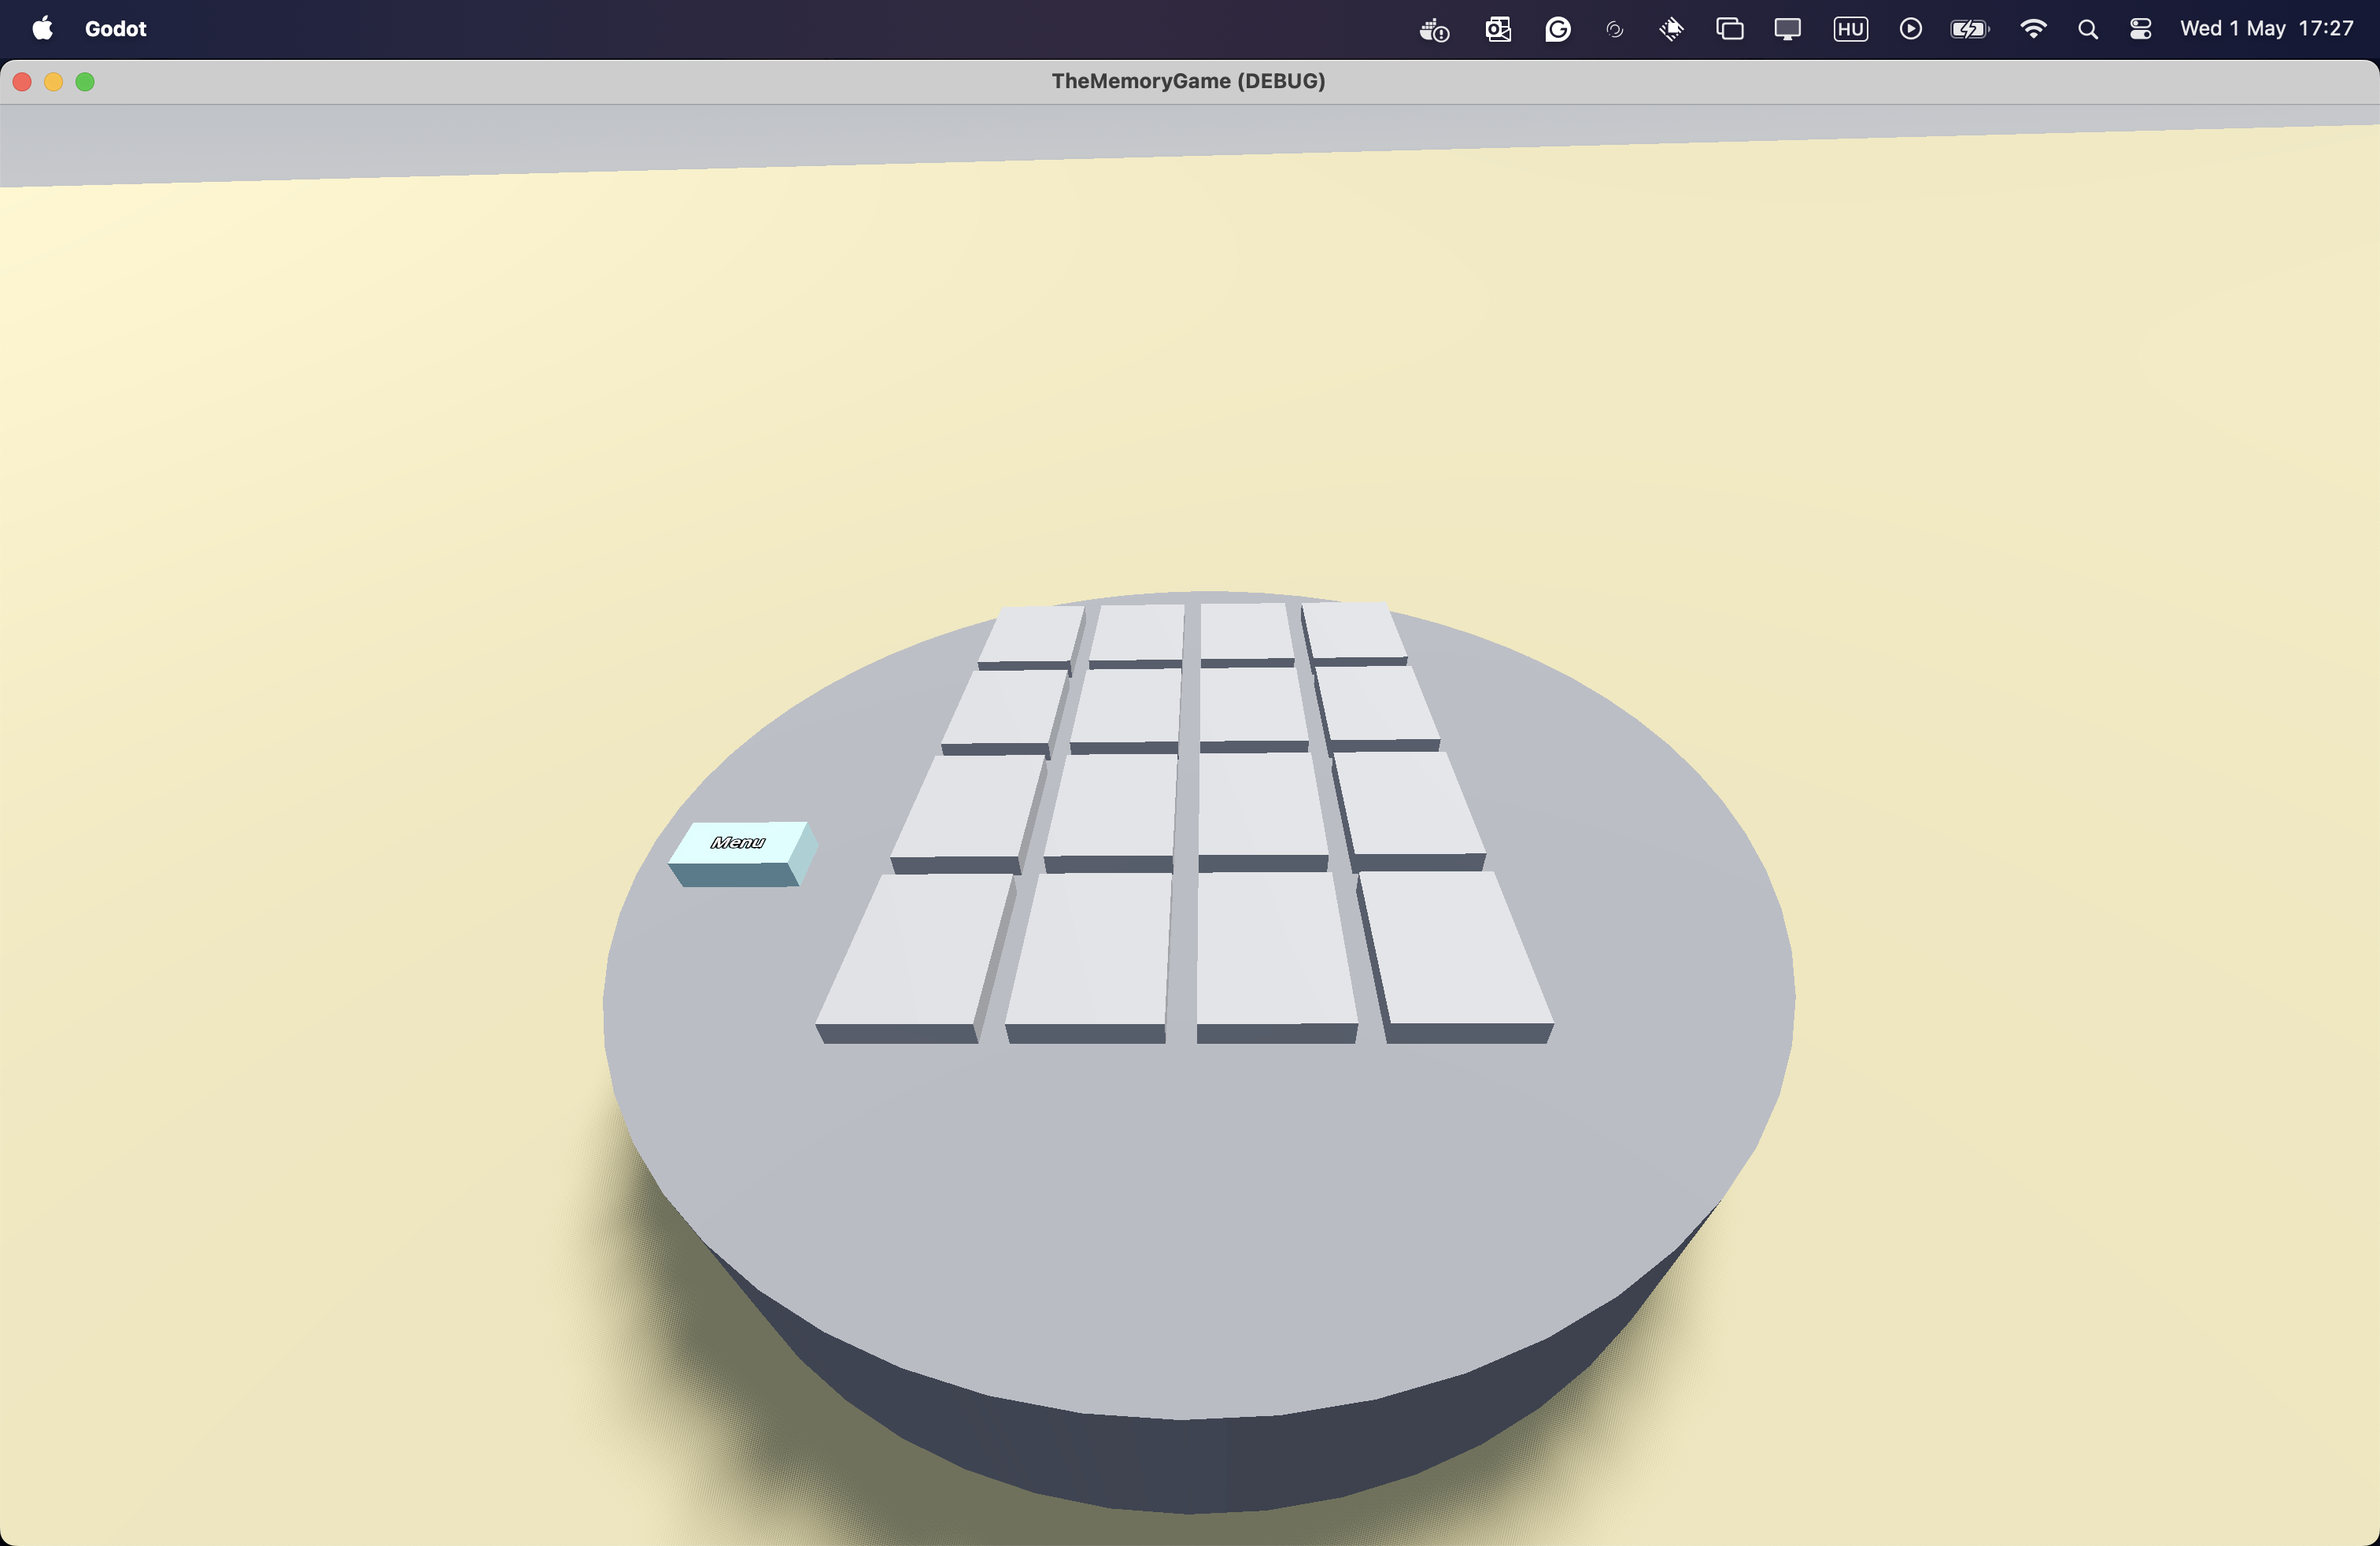
\includegraphics[width=\textwidth]{img/asztal_4x4.png}
    \caption{4x4-es memóriajáték kezdő állapota}
    \label{img:asztal}
\end{figure}
A kártyák előlapján különböző betűk találhatók, minden betűből egy pár. A játékos célja, hogy minél kevesebb kártyapár megfordításából megtalálja az összes memória párt.


A kártya megfordításához a játékosnak rá kell kattintania az adott kártyára. 
Ekkor láthatóvá válik, melyik betű szerepel a memória elemen (\ref{img:kartya_fliped}. ábra). 
Az első választott/megfordított kártyához választani kell egy másikat. A játékosnak törekednie kell, hogy korábbi ismeretei alapján, a következőre a választott kártya előlapján ugyanaz a betű szerepeljen, mint a már felfordított memória lapon, azaz párokat találjon.
Értelemszerűen ez az első felfordításkor csak véletlentszerűen lehetséges, hiszen nincs korábbi ismerete a játékról (\ref{img:non_pair}. ábra).
\begin{figure}[h]
\begin{subfigure}[t]{0.5\textwidth}
    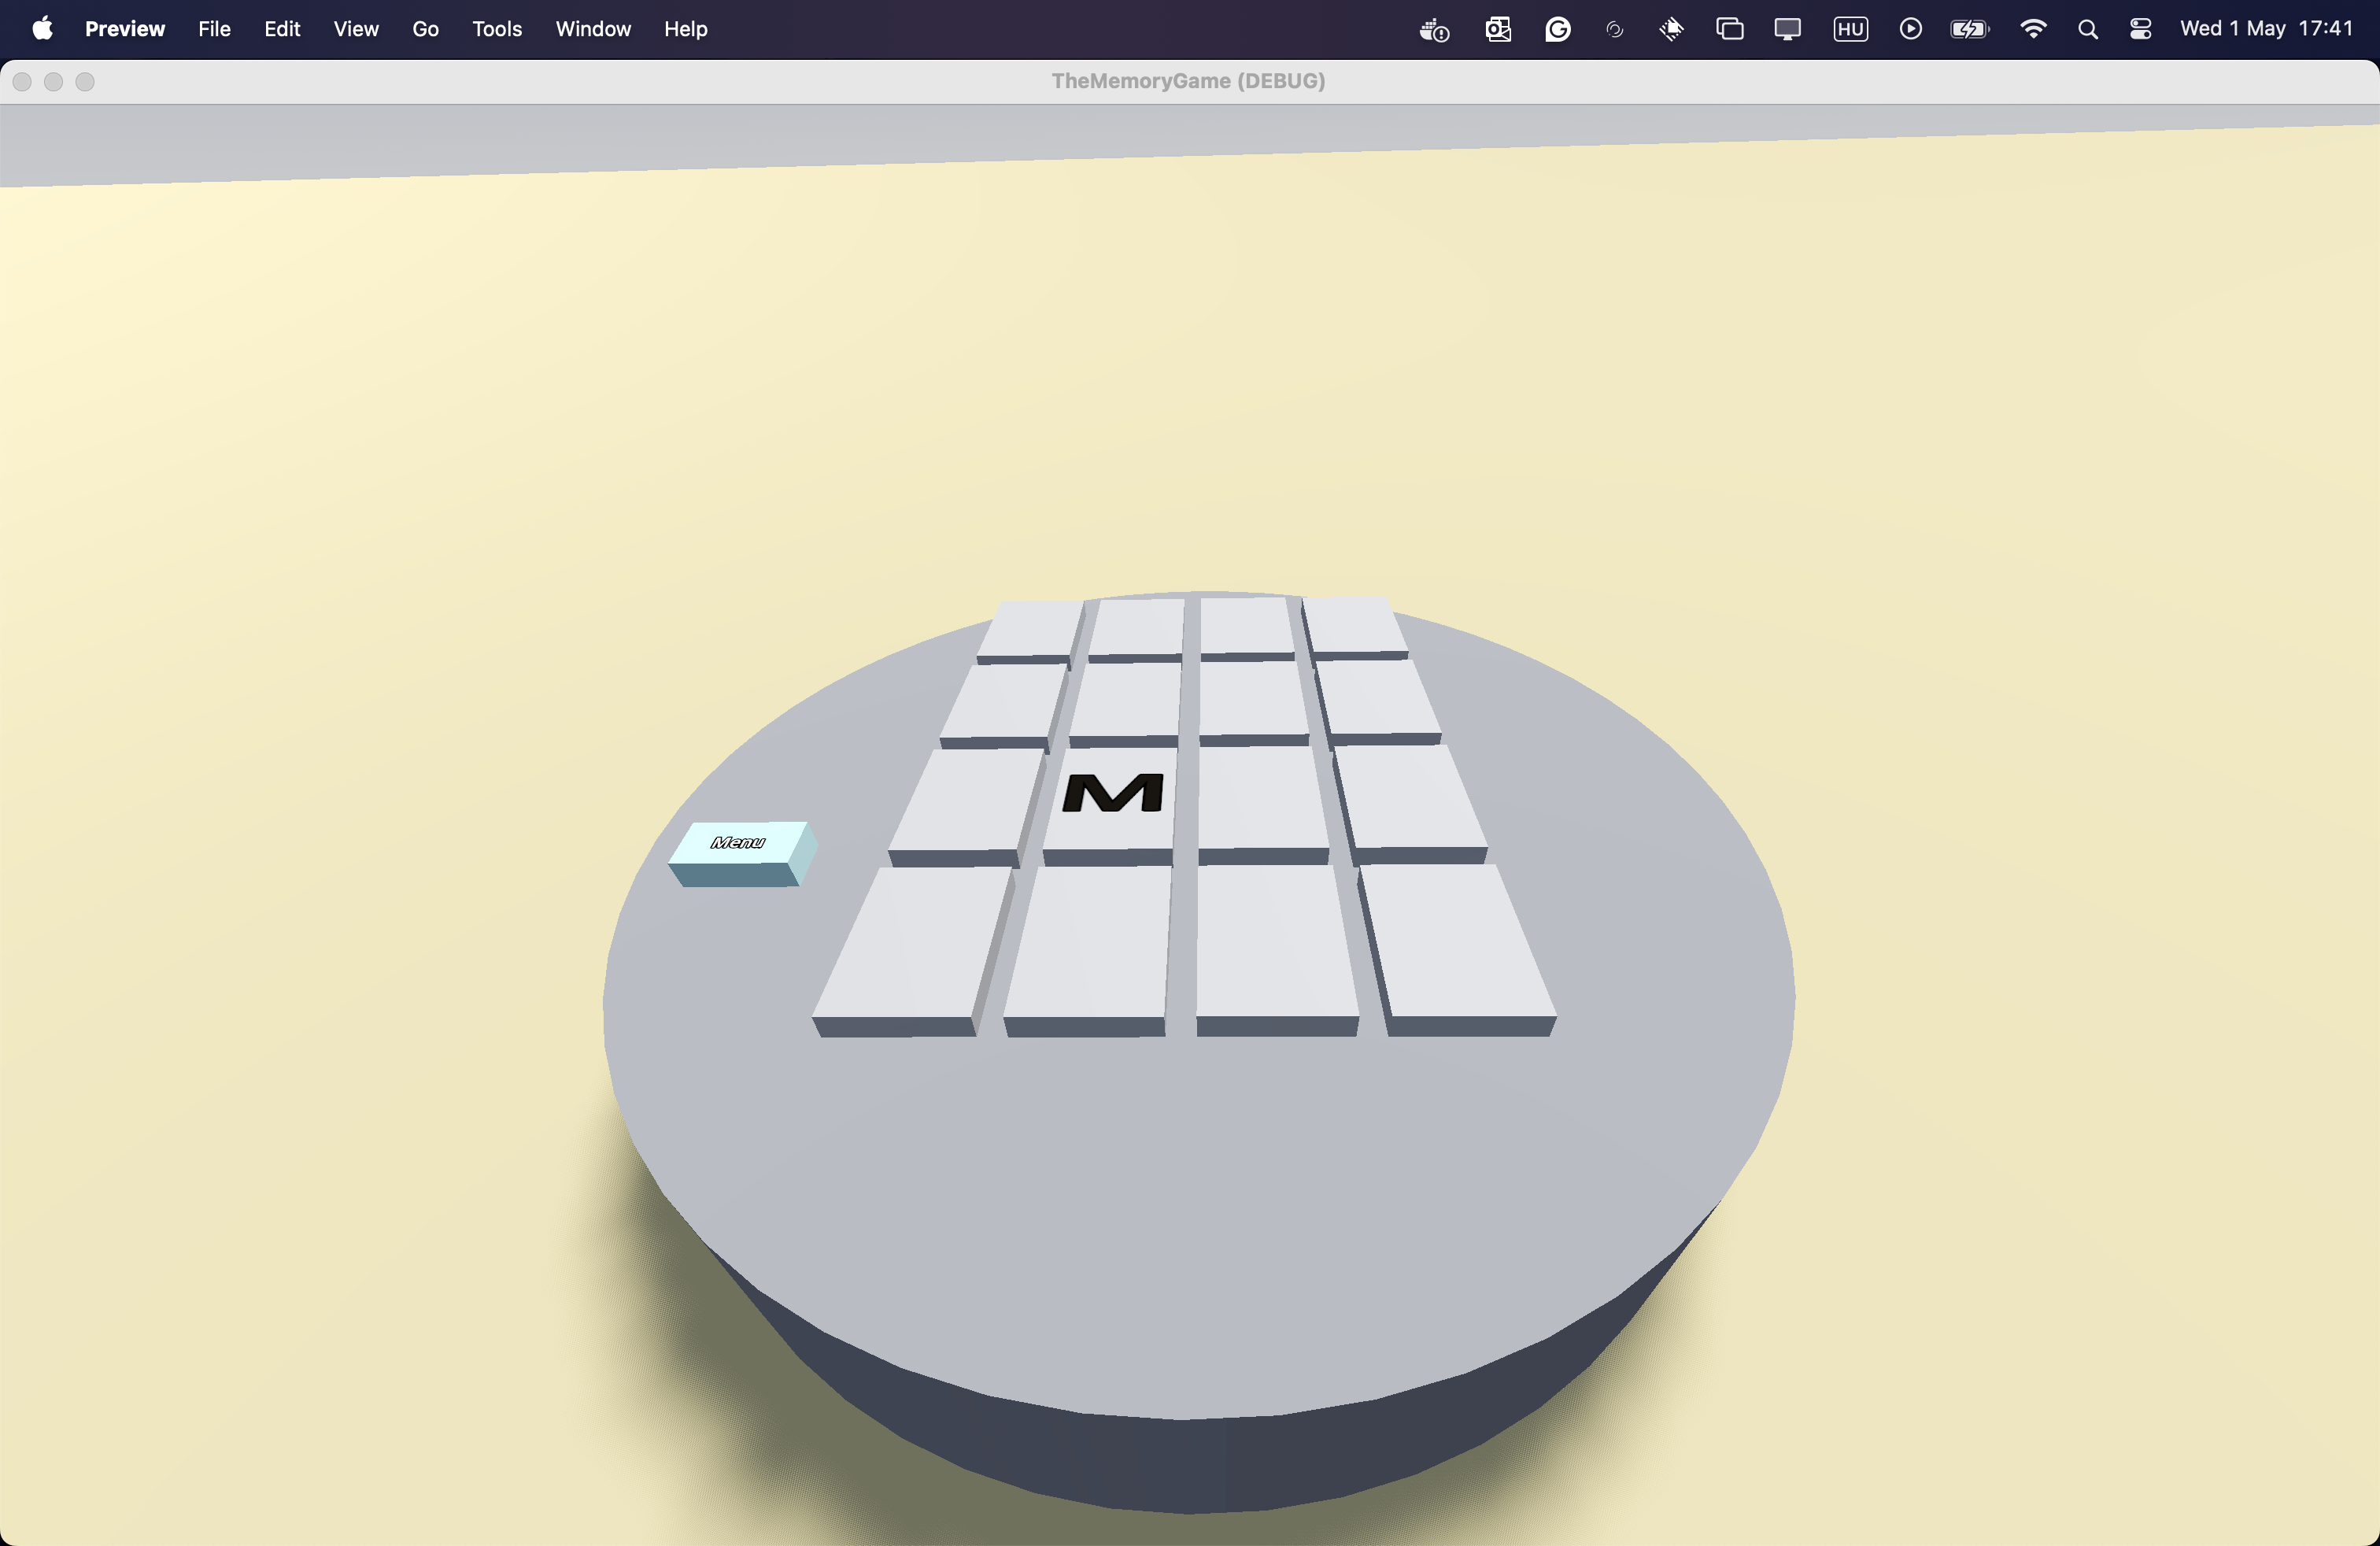
\includegraphics[width=\linewidth]{img/asztal_4x4_card_flipped.png}
    \caption{Egy kártya ki van választva}
    \label{img:kartya_fliped}
\end{subfigure}
\begin{subfigure}[t]{0.5\textwidth}
    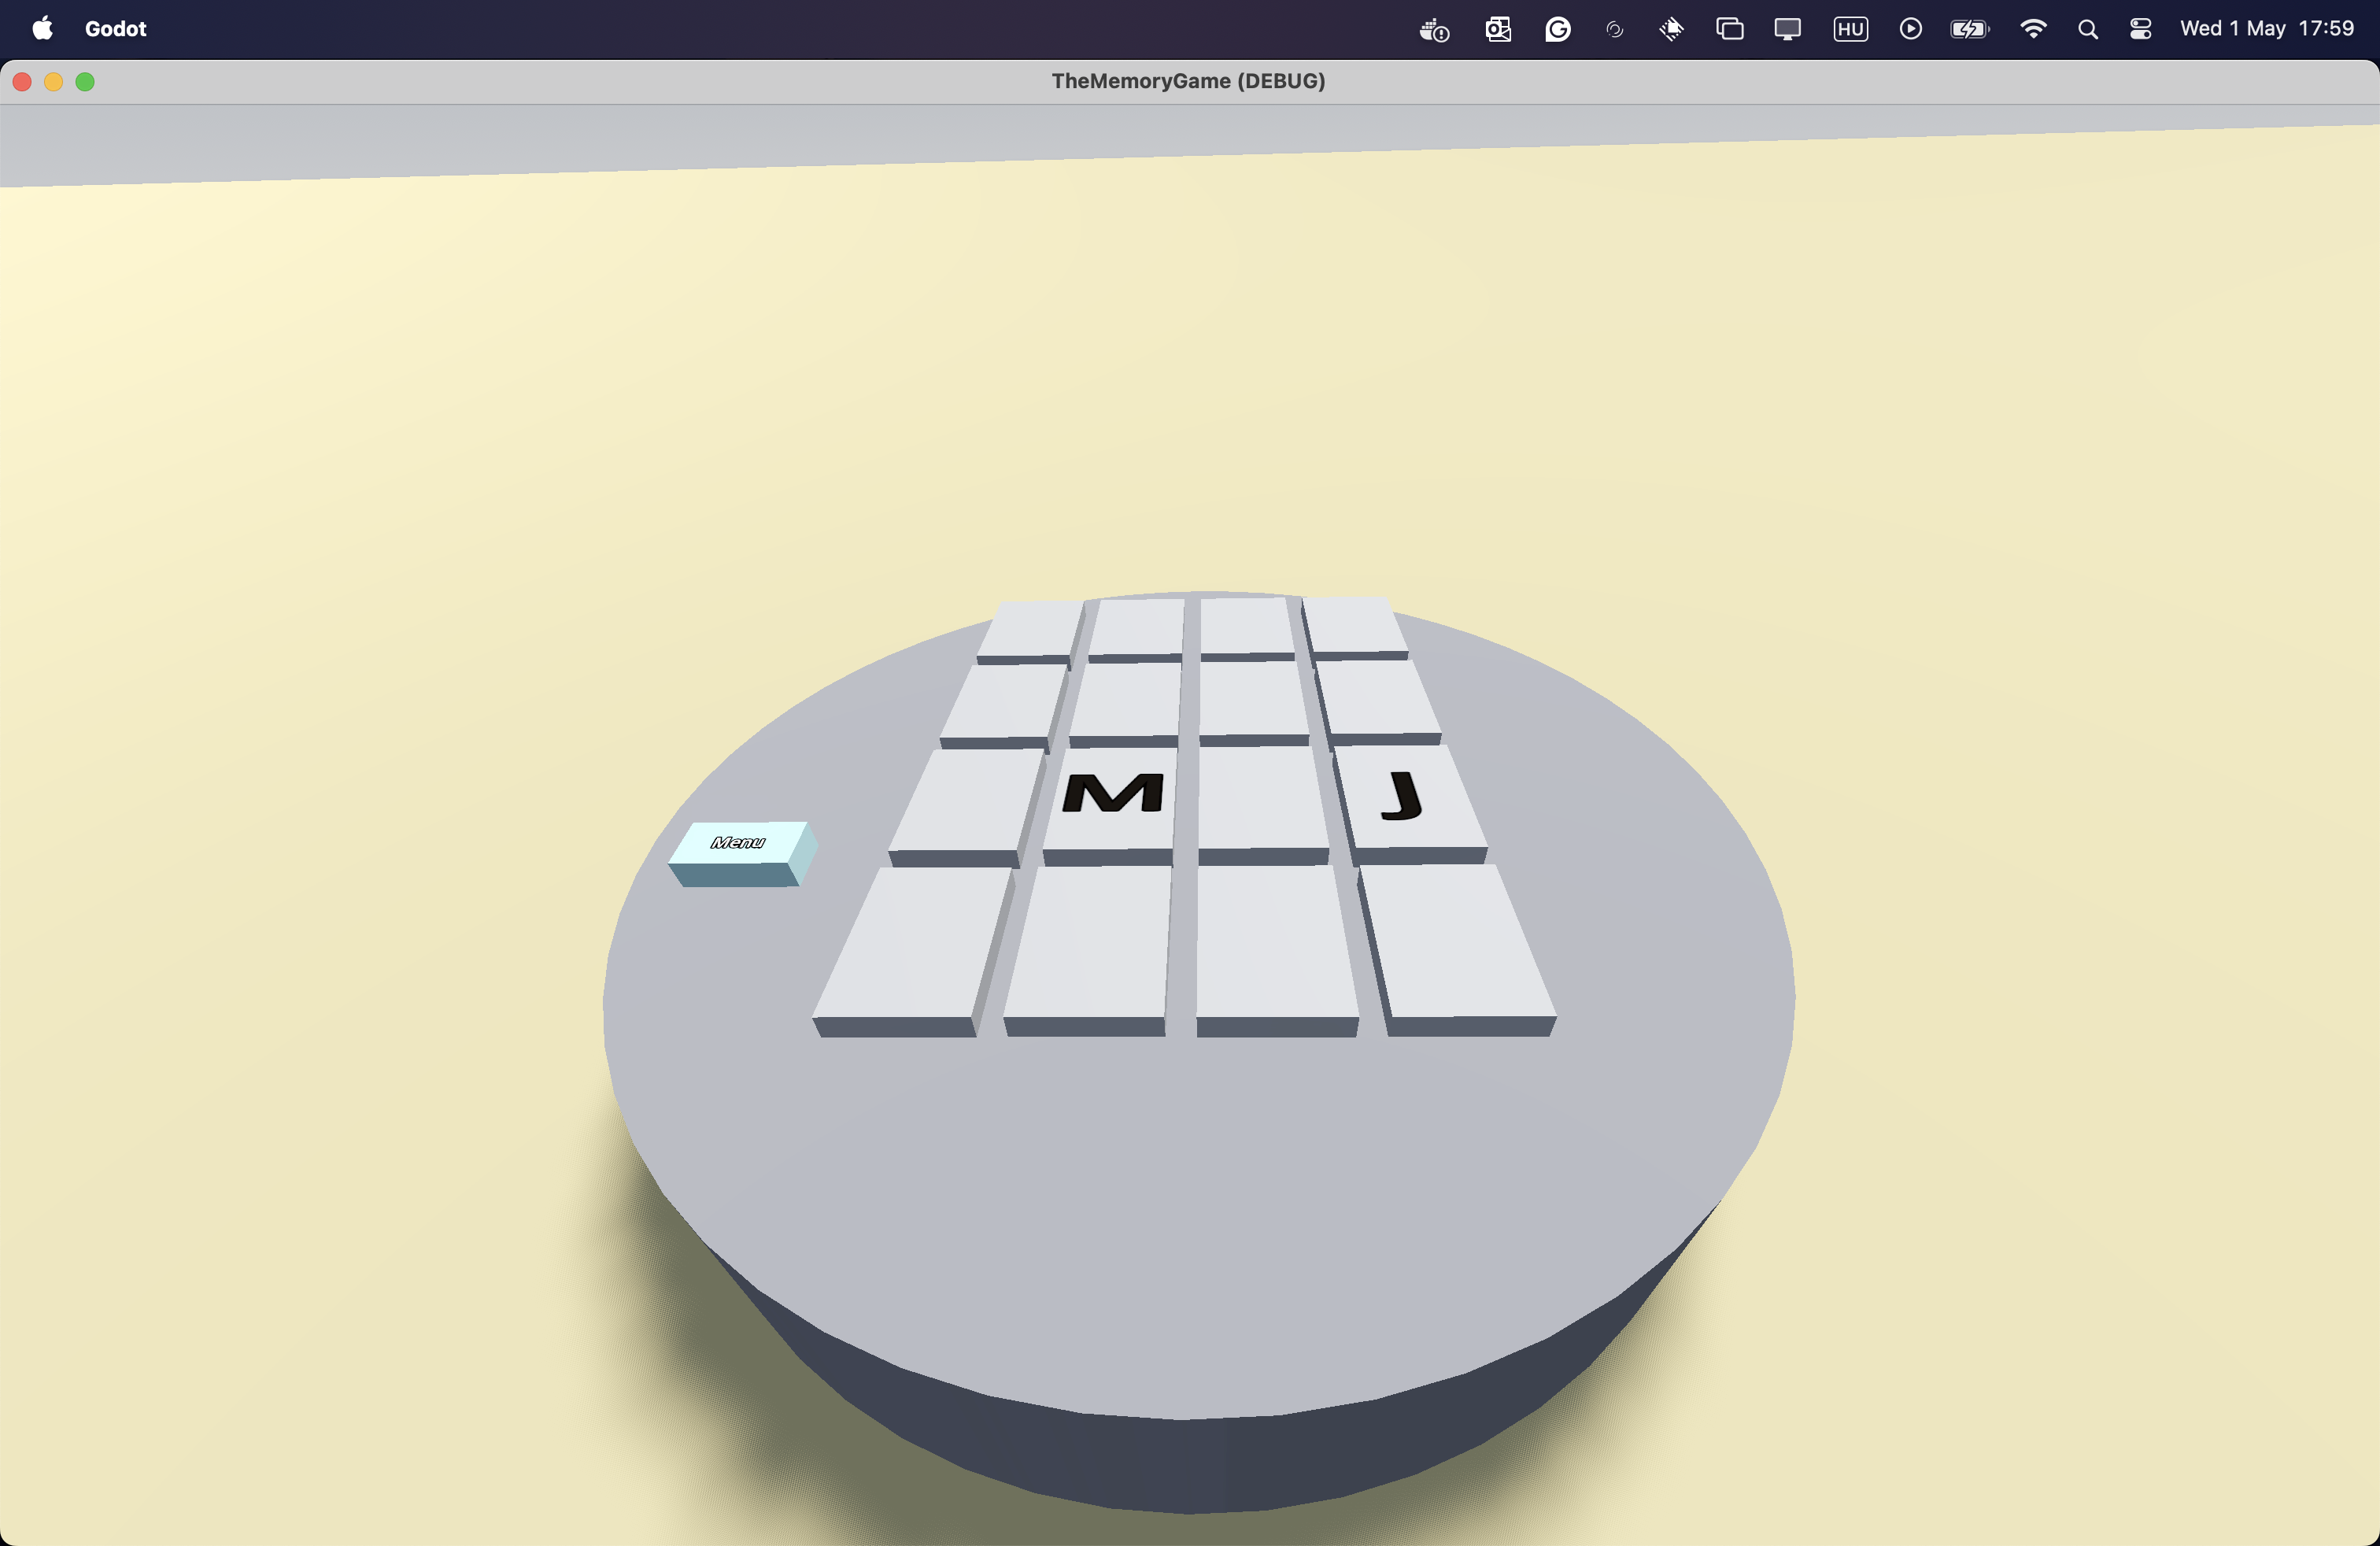
\includegraphics[width=\linewidth]{img/asztal_4x4_non_pair.png}
    \caption{Mivel a betűk nem azonosak, ezér ez nem egy pár, visszafordítjuk a kártyákat.}
    \label{img:non_pair}
\end{subfigure}
\caption{4x4-es játék, példa kör, amikor nem egy párt húzunk fel}
\end{figure}
Ha a felfordított kártyák nem alkotnak párt, akkor a kártyák maguktól visszafordulnak pár másodperc elteltével. Ez után végrehajtunk egy újabb fordítást.
Ha párt alkotnak (\ref{img:pair}. ábra), akkor a kártyák eltűnnek a játékmezőről  (\ref{img:pair_gone}. ábra).
\begin{figure}[H]
    \begin{subfigure}[ct]{0.5\textwidth}
        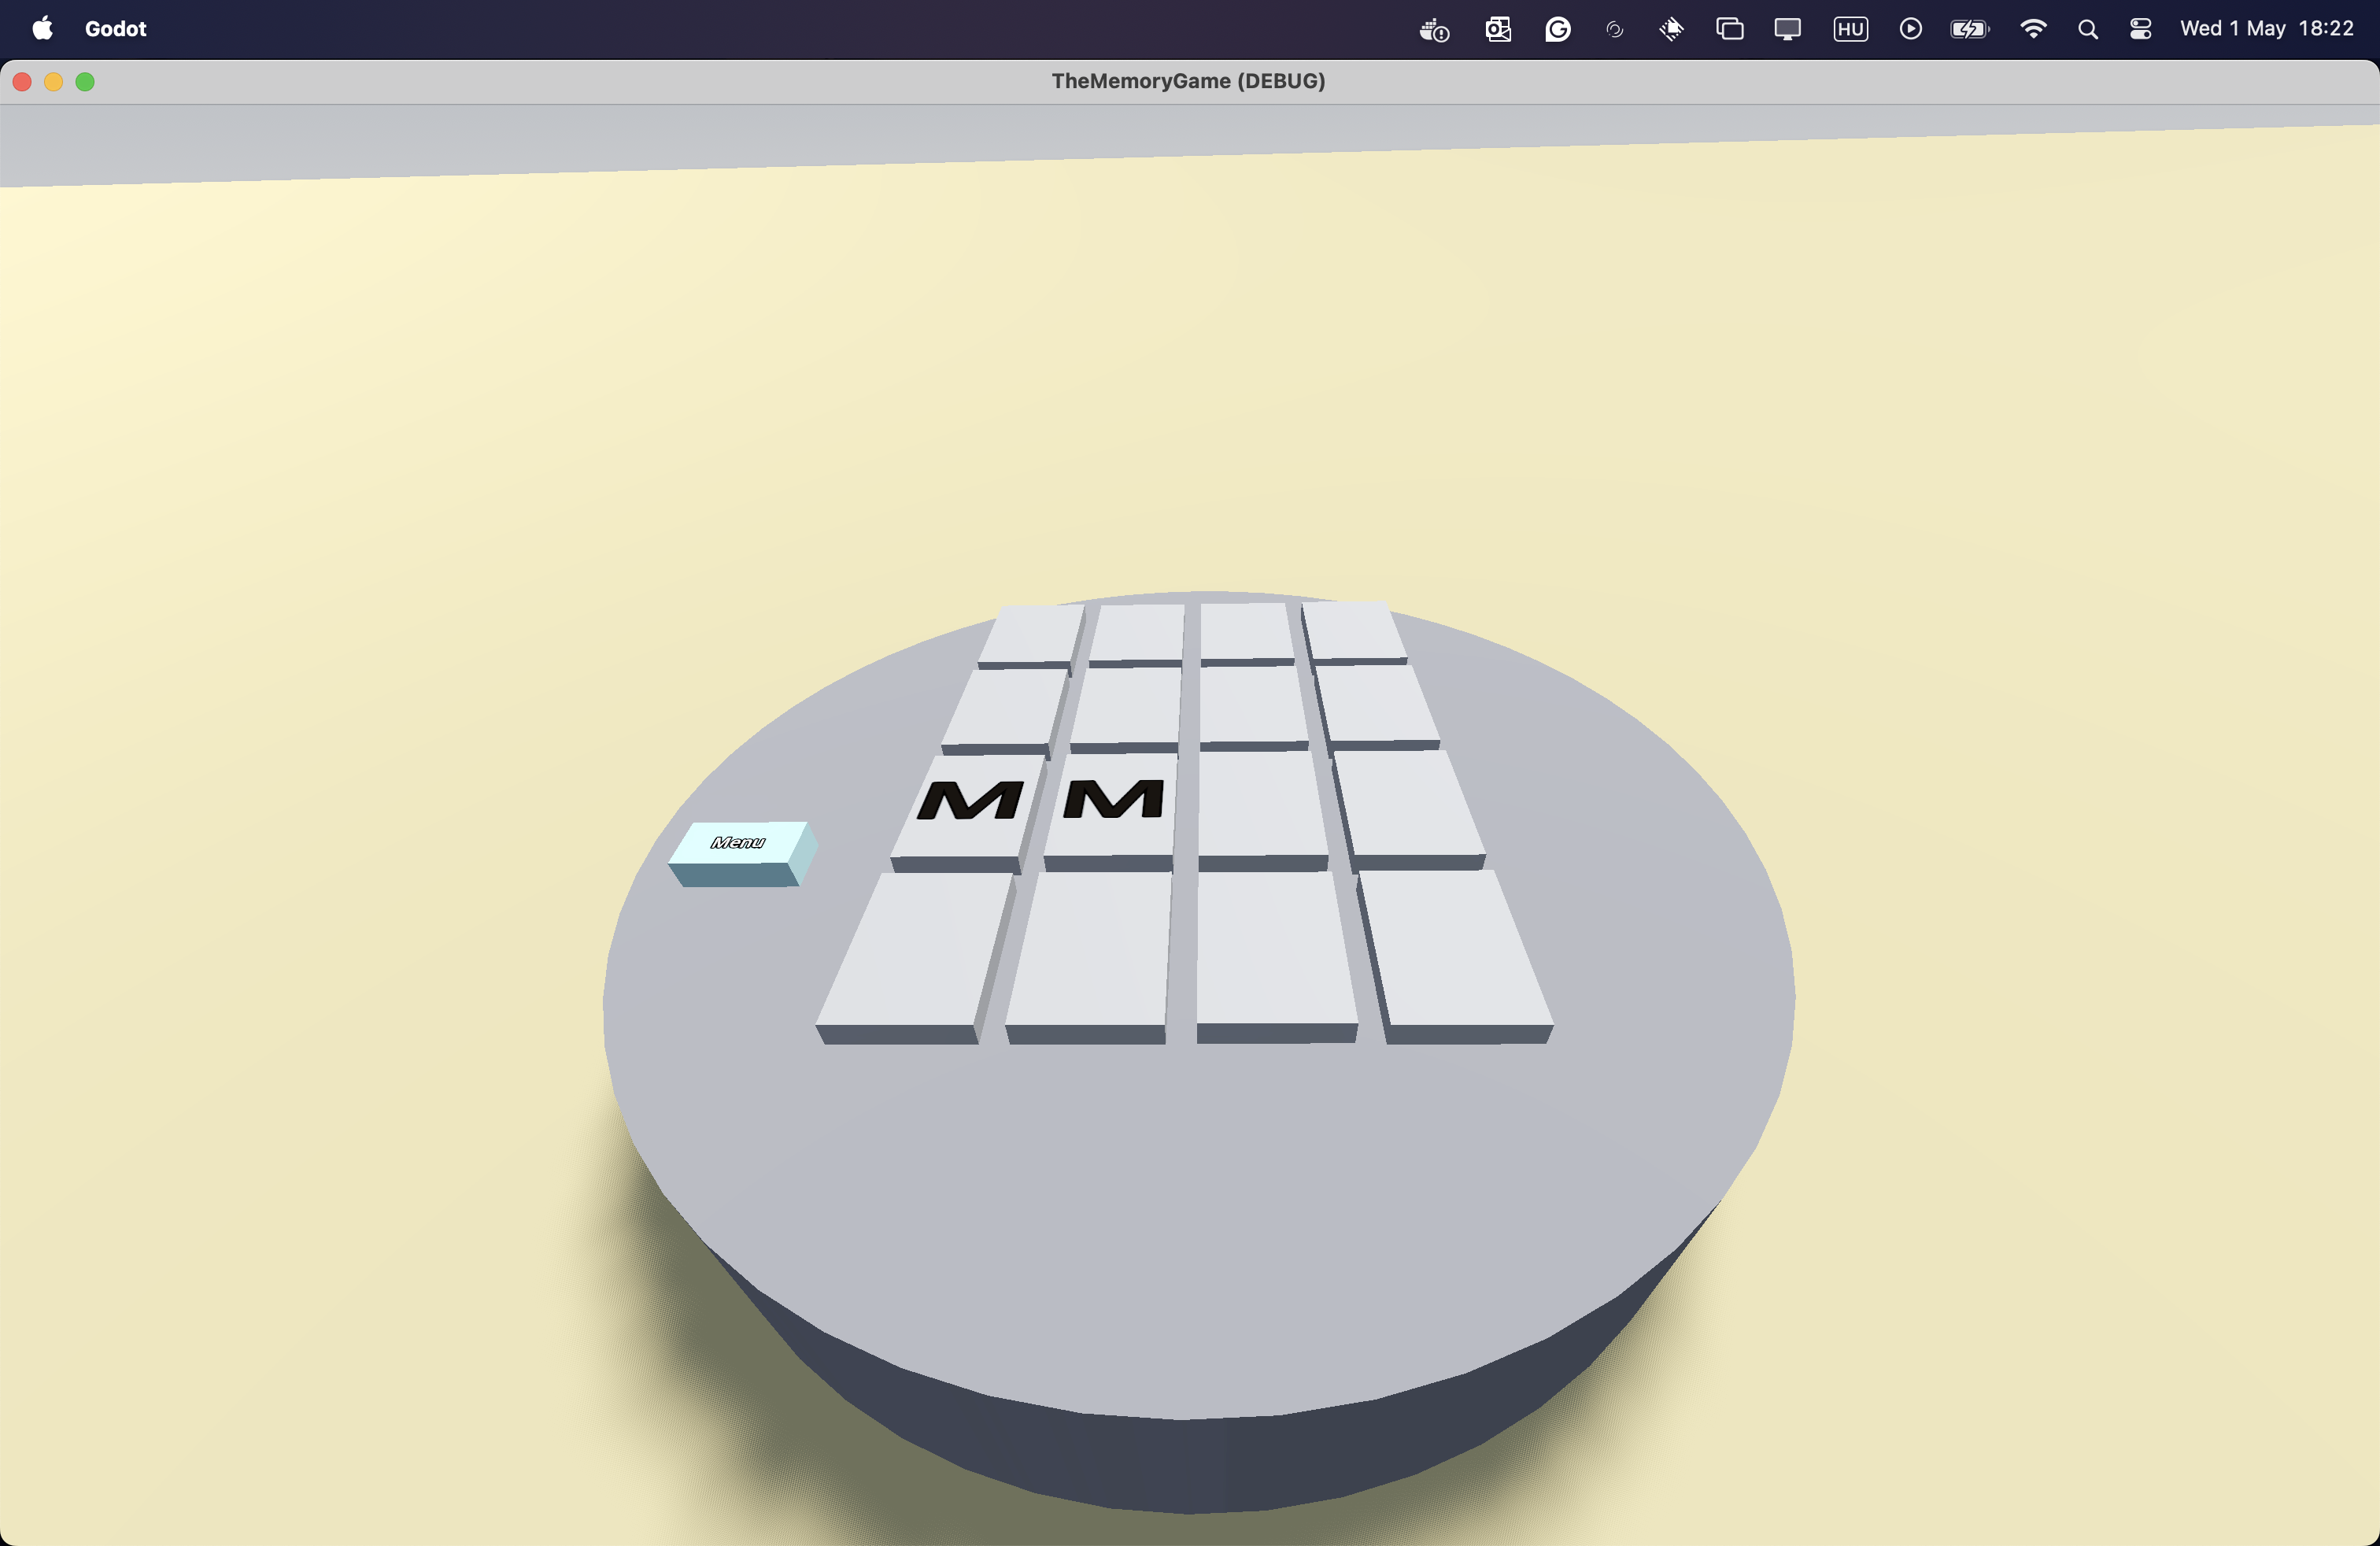
\includegraphics[width=\textwidth]{img/asztal_4x4_pair.png}
        \caption{A kiválasztott kártyák párt alkotnak}
        \label{img:pair}
    \end{subfigure}
    \begin{subfigure}[ct]{0.5\textwidth}
        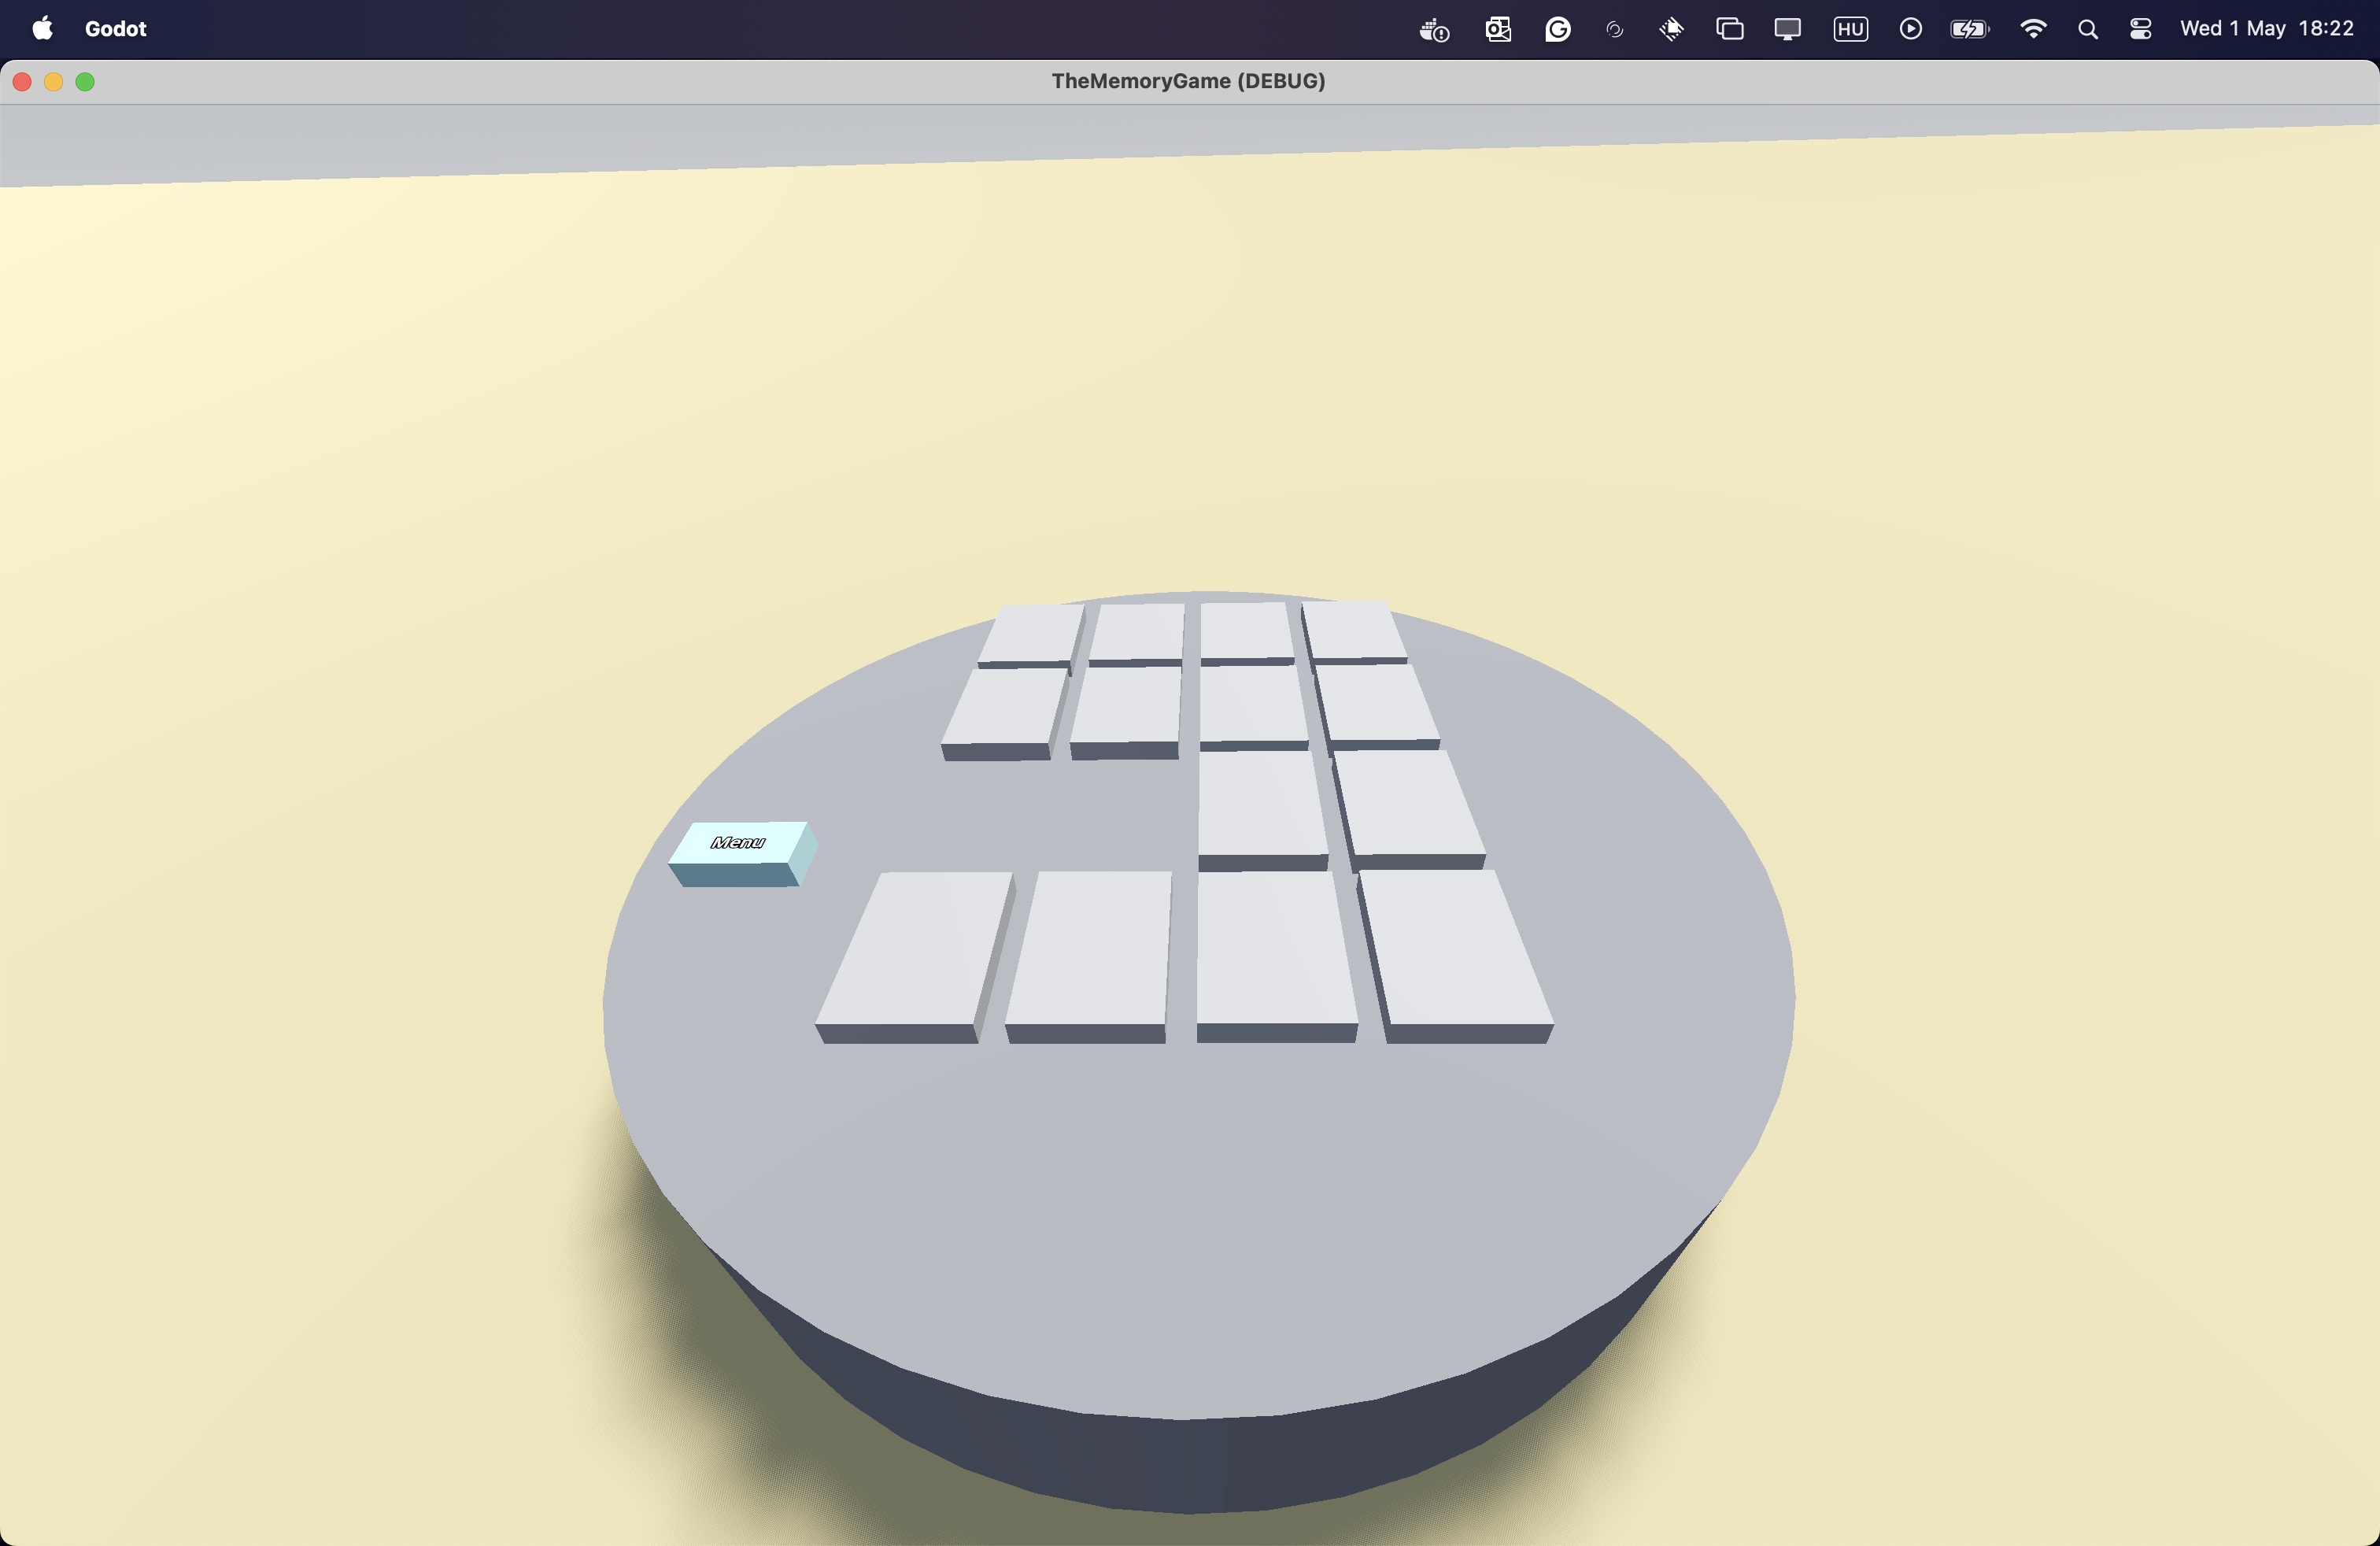
\includegraphics[width=\textwidth]{img/asztal_4x4_pair_eltunik.png}
        \caption{Eltűnik a pár az asztalról}
        \label{img:pair_gone}
    \end{subfigure}
    \caption{4x4-es játék, példa kör, amikor egy párt húzunk fel}
\end{figure}


Amint az összes kártya eltűnik az asztalról, a játék véget ér, és visszakerülünk a menübe.
A játékba több nehézségi szintet tettünk, melyet a menüből érhetünk el (\ref{img:menu}. ábra). A különböző menüpontok, a kártyák számának elhelyezkedését jelölik.
\begin{figure}[h]
    \centering
    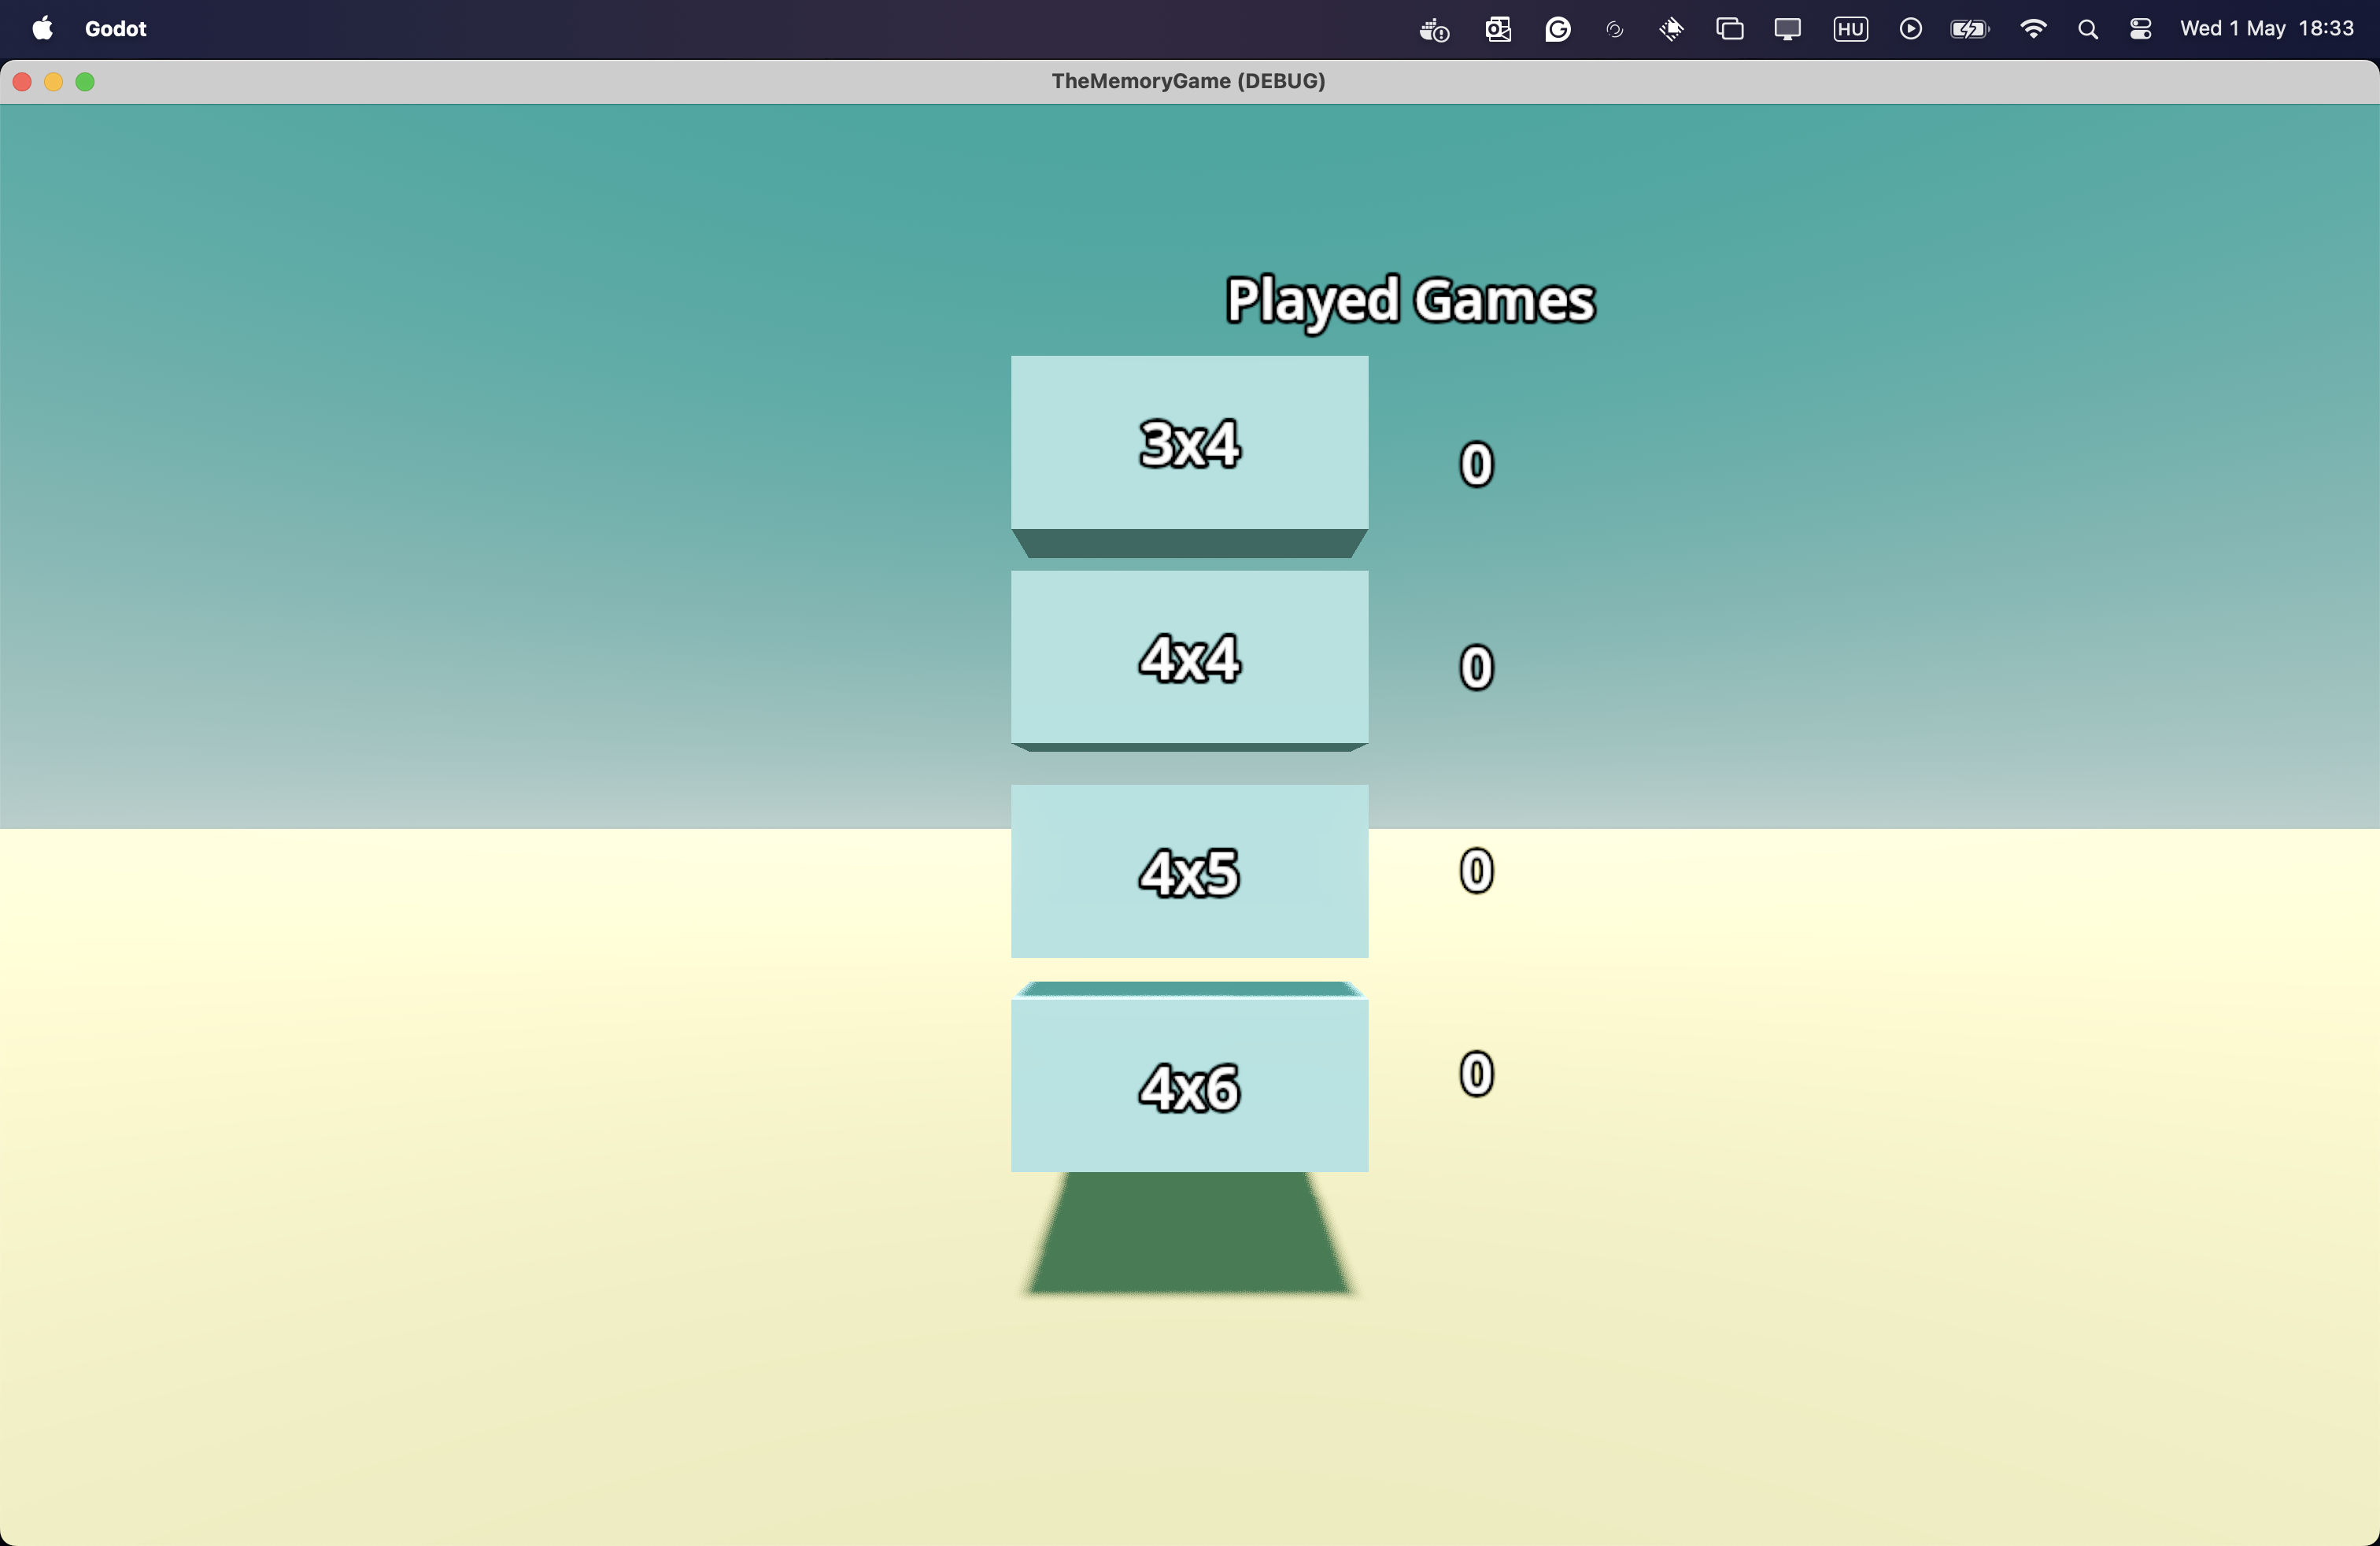
\includegraphics[width=0.5\textwidth]{img/menu.png}
    \caption{A játék menüje}
    \label{img:menu}  
\end{figure}

\section{Struktúrális felépítés}
A memória játék a Godot elveinek megfelelően Node-okból és Scene-ekből \cite{godotengineNodesScenes} áll. A Scene-ek struktúrája a következő.
\subsection{Menü}


A Játék menüje (\ref{img:menu_scene}. ábra), a következő módon épül fel. A Gombok olyan MeshInstance3D Node-ok \cite{godotengineMeshInstance3D}, melyekre ha a játékos rákattint, akkor emittálnak egy \lstinline{button_pressed()} signal-t (\ref{code:button_pressed_signal}. ábra).
A MenuScene kódjában hallgatózunk erre a signal-ra, külön külön minden gombokra. A megfelelő gomb megnyomásával beállítjuk a \lstinline{Constant.CARD_PMIR_NUMBER} globális változót, melynek segítségével létrehozzuk a \lstinline{basic_scene}-t.
\begin{figure}[h]
    \centering
    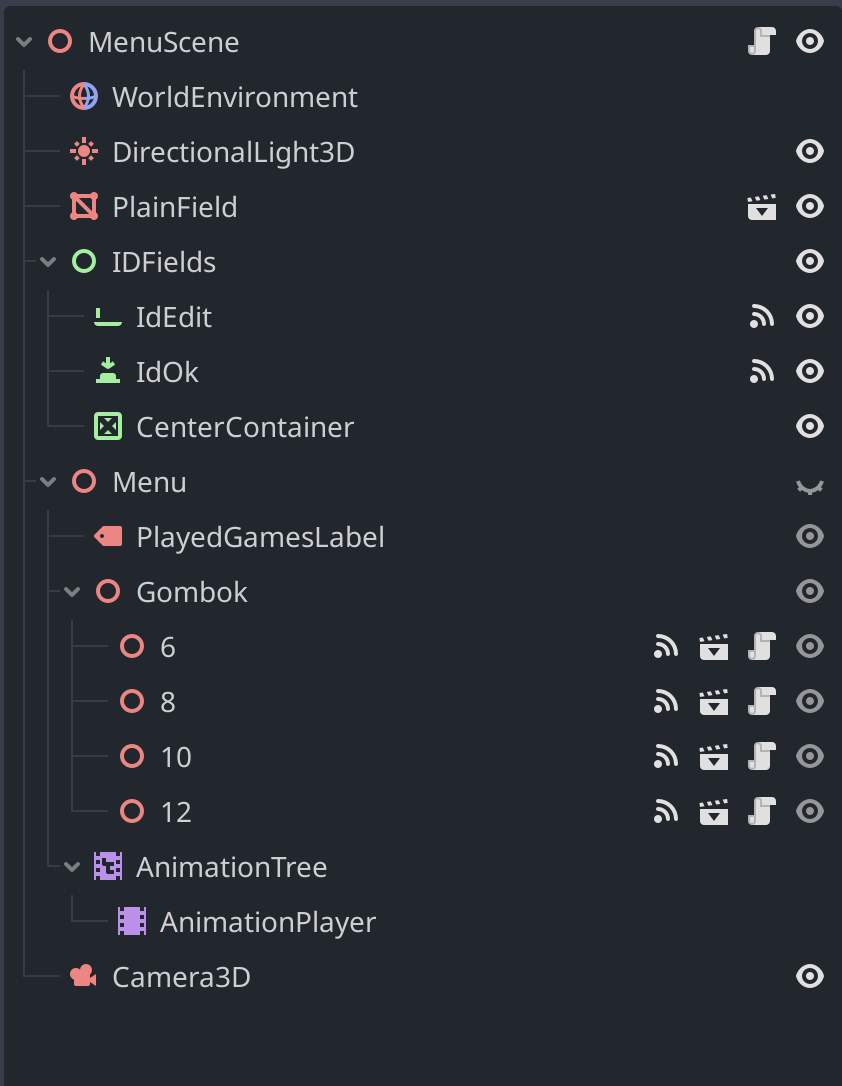
\includegraphics[width=0.5\textwidth]{img/menu_scene_tree.png}
    \caption{A játék menü Scene-jének struktúrája}
    \label{img:menu_scene}  
\end{figure}

\begin{figure}[H]
    \centering
    \begin{lstlisting}[language=GDScript]
    func _on_area_3d_input_event(camera, event, position, normal, shape_idx):
        if event is InputEventMouseButton:
            if (event.button_index == MOUSE_BUTTON_LEFT && event.pressed == true):
                emit_signal("button_pressed")
    
    func set_number_label_text(new_label_text: String):
        number_label.text = new_label_text;
    \end{lstlisting}
    \caption{A menü gombja  \lstinline{button_pressed} signal-t emittál}
    \label{code:button_pressed_signal}
\end{figure}

\subsection{Basic Scene}

A Basic Scene (\ref{img:basic_scene}. ábra) struktúrája dinamikusan épül fel a \lstinline{Card} Scene-ekből, melyet a \lstinline|Deck| globális objektum ad oda a \lstinline|Basic Scene| -nek. 
\begin{figure}[H]
    \centering
    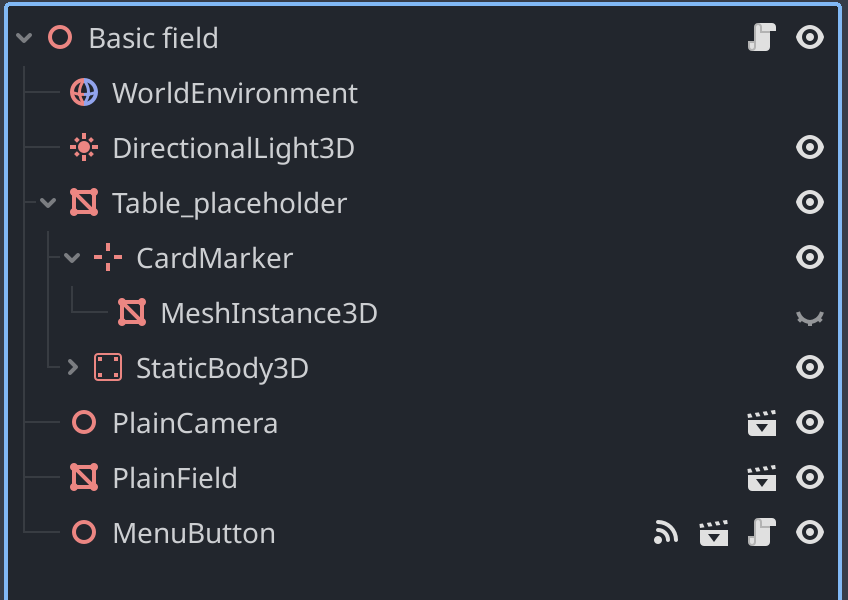
\includegraphics[width=0.5\textwidth]{img/basic_field_scene_structure.png}
    \caption{A játéktér Scene struktúrális felépítése}
    \label{img:basic_scene}  
\end{figure}

A scene kiszámolja, az előre beállított kártyaszélesség, -magasság és -margó konstansok alapján, hogy a megkapott darabszámú kártyát, a \lstinline|CardMarker| -höz képest hova kell lerakni (\ref{code:calculate_coordinate}. ábra)
\begin{figure}[H]
    \centering
    \begin{lstlisting}[language=GDScript]
        func _calculate_coordinate(i, j):
        return Vector3(
            TABLE.position.x + (((CARD_WIDTH  + MARGO) * CARD_SCALE) * i ) - (((CARD_WIDTH * CARD_ROW) - (CARD_WIDTH) + (MARGO*(CARD_ROW-1)))*CARD_SCALE / 2),
            TABLE.position.y,
            TABLE.position.z + (((CARD_HEIGHT  + MARGO) * CARD_SCALE) * j ) - (((CARD_HEIGHT * CARD_COLUMN) - (CARD_HEIGHT) + (MARGO*(CARD_COLUMN-1)))*CARD_SCALE / 2)
        )
    \end{lstlisting}
    \caption{Kártyák koordinátájának kiszámítása}
    \label{code:calculate_coordinate}
\end{figure}
Amint a \lstinline|Deck| objektum elküldi a \lstinline{cards_empty} signal-t, vagyis a játék végét, vagy ha a játékos megnyomja a Menü gombot, a játék visszatér a menübe. 

Más feladata nincs. 


\subsection{Deck}
A \lstinline|Deck| egy olyan globális objektum, mely a program futása során bármikor elérhető. A feladatai: 
\begin{enumerate}
\item Létrehozni a kártyákat, a játék kezdetekor (\ref{code:make_deck}. ábra)
\item Folyamatosan figyeli, hogy mely \lstinline|Card|-ok vannak még játékban a lstinline|cards| tömbben.
\item Kezeli a kártyák felfordítását. Ha két kártya azonos, akkor azokat kiveszi a listájából (\ref{code:talalat}. ábra).
\item Lementeni a játékos minden lépését a data tömb változóba, a memóriába. 
\item Figyeli a játék végét.
\item Lementeni a data tömböt egy JSON file-ba a játék végével.
\end{enumerate}

\begin{figure}[h]
    \centering
    \begin{lstlisting}[language=GDScript]
    func make_deck(card_pair_number: int, card_scene: PackedScene):
        data.card_pair_number = card_pair_number;
        cards.clear();
        for i in range(0, card_pair_number):
            var word = "";
            while ABC.find(word) > - 1 or word == "":
                word = generate_word('abcdefghijklmnopqrst', 1).to_upper();
            ABC.push_back(word);
            var card = card_scene.instantiate();
            #call_deferred("add_child", card);
            if card.has_method("set_label"):
                card.set_label(word);
            cards.push_back(card);
            cards.push_back(card.duplicate());
        cards.shuffle();
        data.card_labels = ABC;
    \end{lstlisting}
    \caption{Létrehozzuk a kártyákat}
    \label{code:make_deck}
\end{figure}
\begin{figure}[h]
    \centering
    \begin{lstlisting}[language=GDScript]
func talalat():
	if (chosenA.get_label() == chosenB.get_label()):
		cards.remove_at(cards.find(chosenA));
		cards.remove_at(cards.find(chosenB));
		chosenA.queue_free();
		chosenB.queue_free();
	else:
		chosenA.play_card_reflip_animation();
		chosenB.play_card_reflip_animation();
	chosenA = null;
	chosenB = null;
	can_flip = true;
	if cards.size() == 0 :
		cards_empty.emit()
		save_data()
    \end{lstlisting}
    \caption{Figyeljük a találatot}
    \label{code:talalat}
\end{figure}


\subsection{Card}
A kártyák vagyis Card scene (\ref{img:card_tree}. ábra) rendelkezik egy \lstinline|labellel| amelyet a \lstinline|Deck| ad neki, a kártya létrehozásakor. Ez meghatározza, hogy milyen kártya. 
Egy játékmezőn pontosan két egyforma labellel rendelkező kártya szerepel(\ref{img:cards_has_pairs}. ábra).

\begin{figure}[H]
    \centering
    \begin{minipage}[b]{0.45\textwidth}
        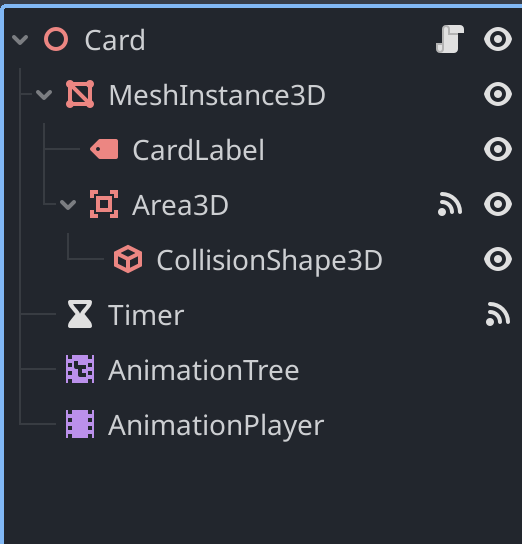
\includegraphics[width=\textwidth]{img/cards_scene_tree.png}
        \caption{A Card Scene struktúrája}
        \label{img:card_tree}
    \end{minipage}
    \hfill
    \begin{minipage}[b]{0.45\textwidth}
        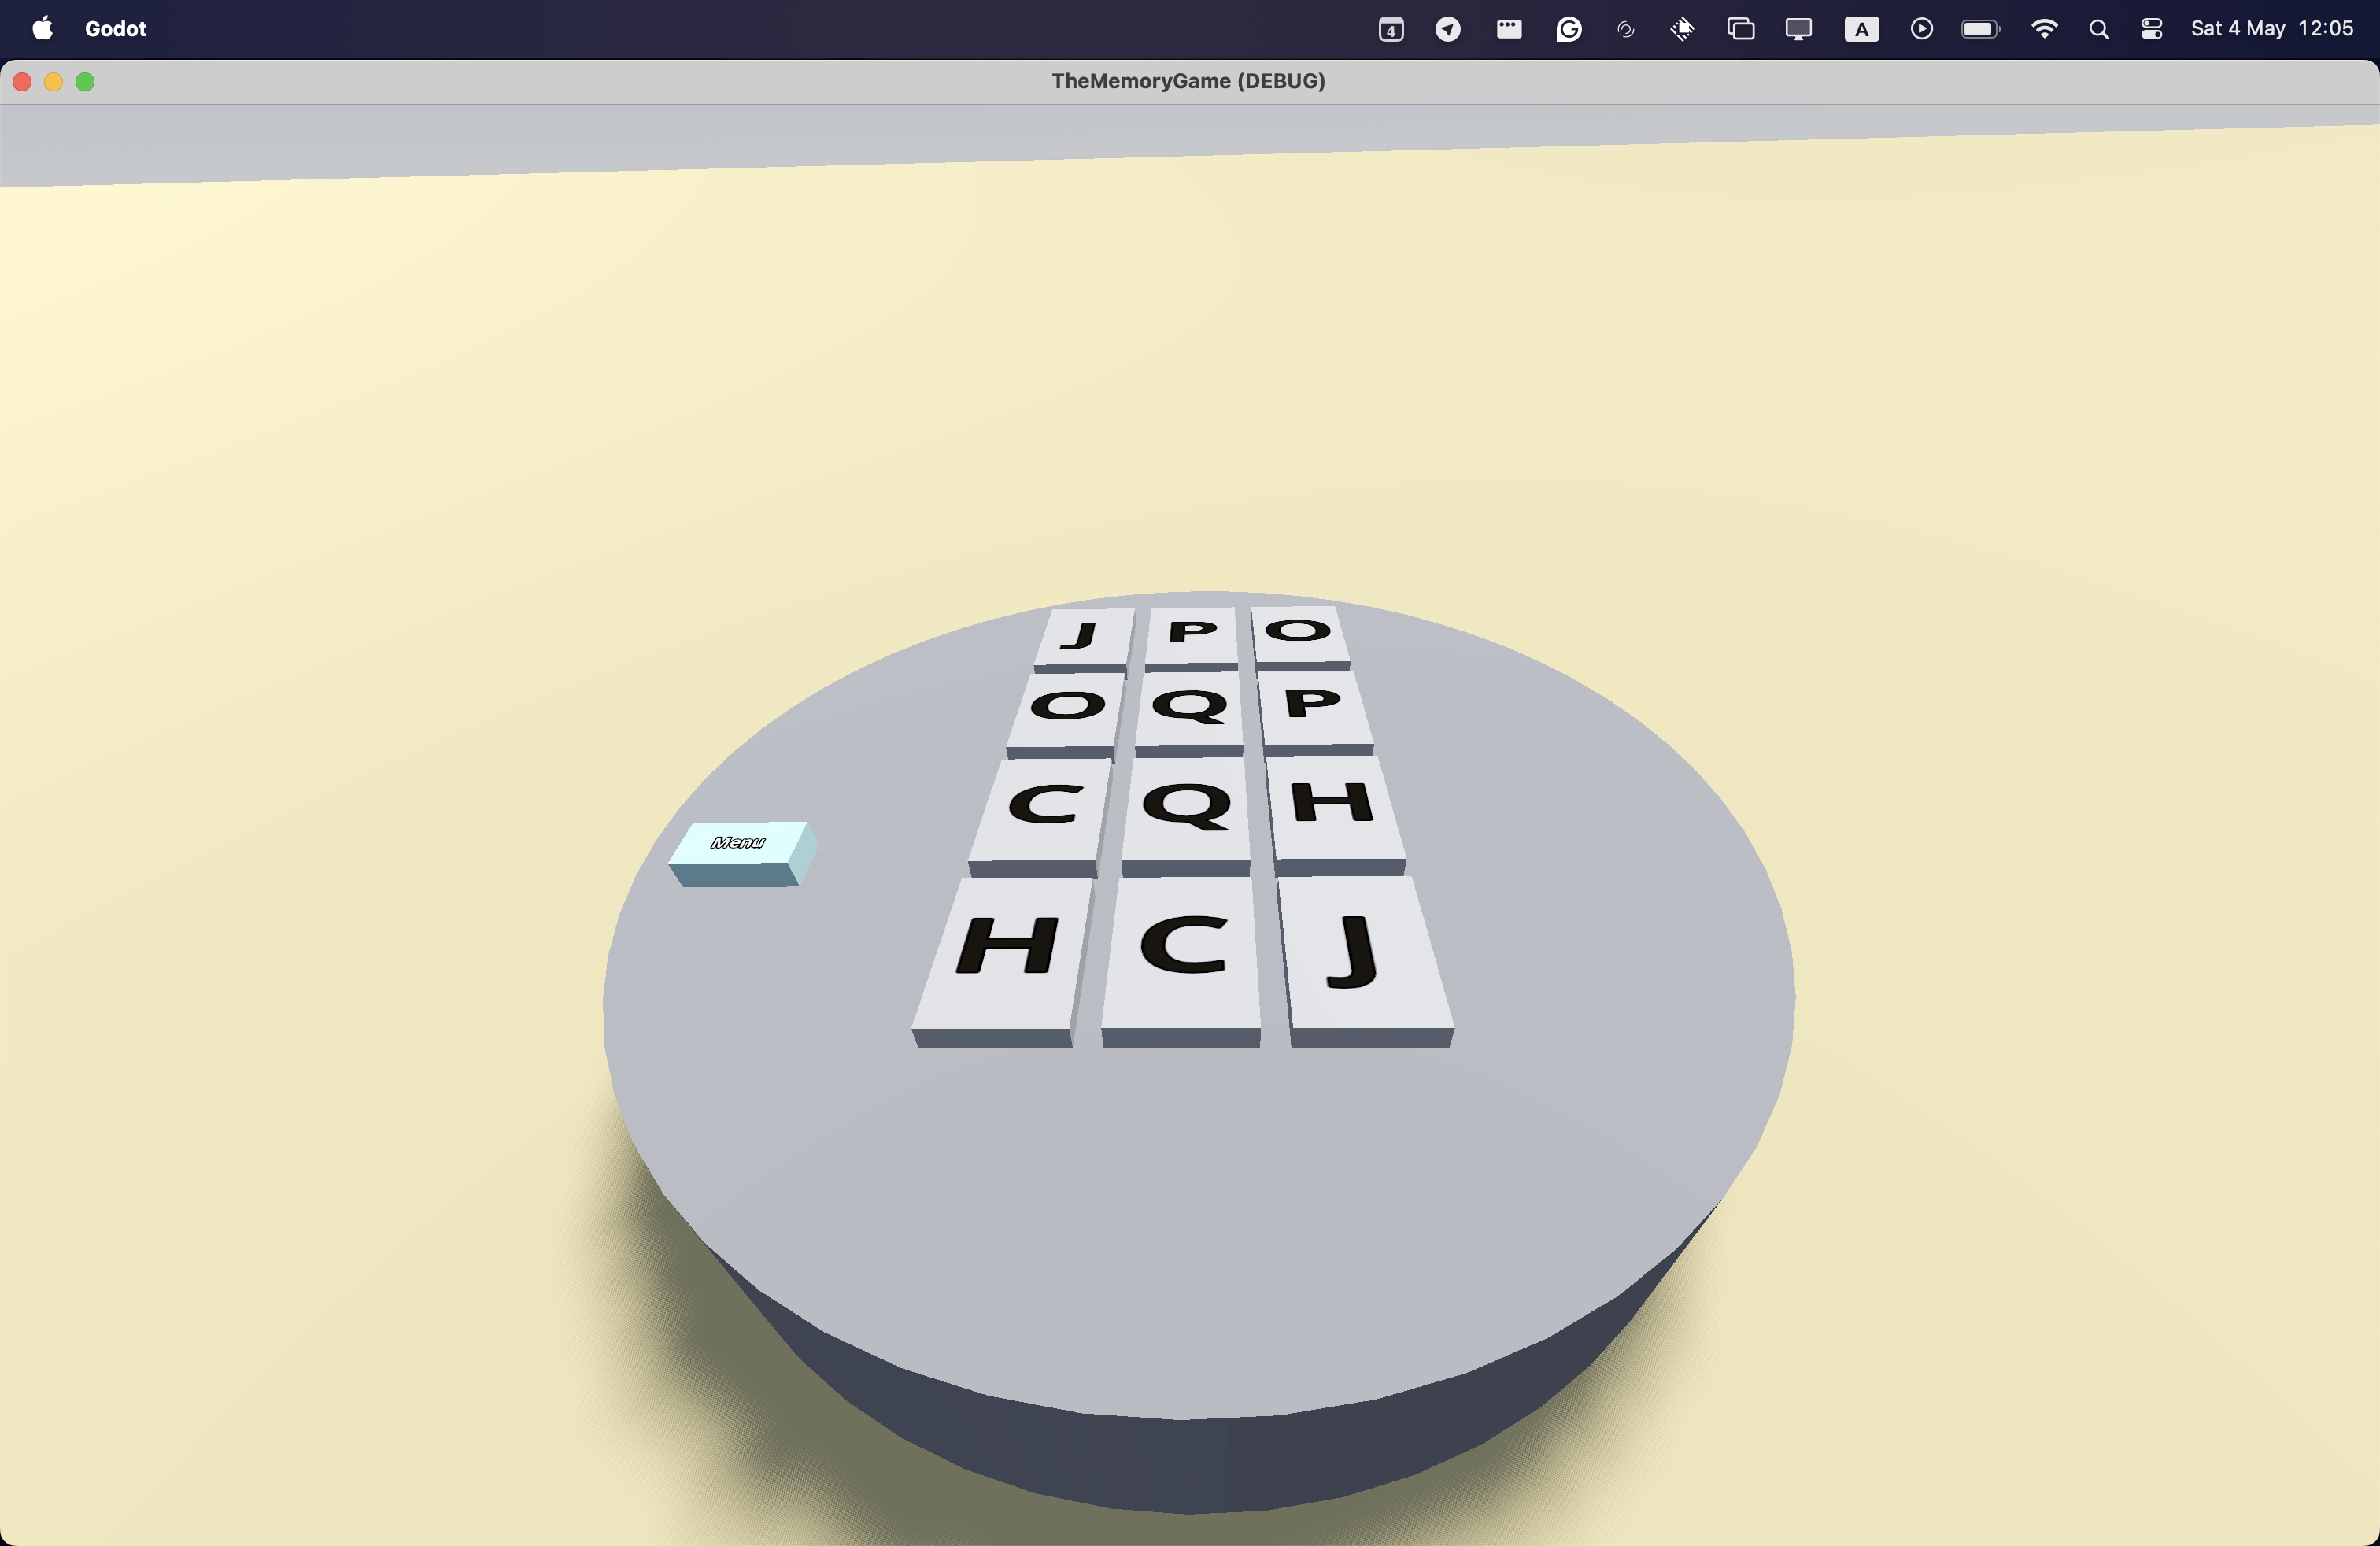
\includegraphics[width=\textwidth]{img/4x4_all_card_fliped.png}
        \caption{4x4 kártya. Minden betűből csak egy pár szerepel}
        \label{img:cards_has_pairs}  
    \end{minipage}
\end{figure}

A kártya rendelkezik animációval is, melyet az AnimationTree (\ref{img:animation_tree}. ábra) kezel. 
Ha rákattintunk a kártyára, akkor lefut a \lstinline|card_flip_animation| function, vagyis az AnimationTree State Machine-nek odaadjuk azt az információt, mely szerint meg kell fordítani a kártyát. Az objektum elküldi önmagát a \lstinline|Deck|-nek, mint kiválasztott kártya. 
\begin{figure}[h]
    \centering
    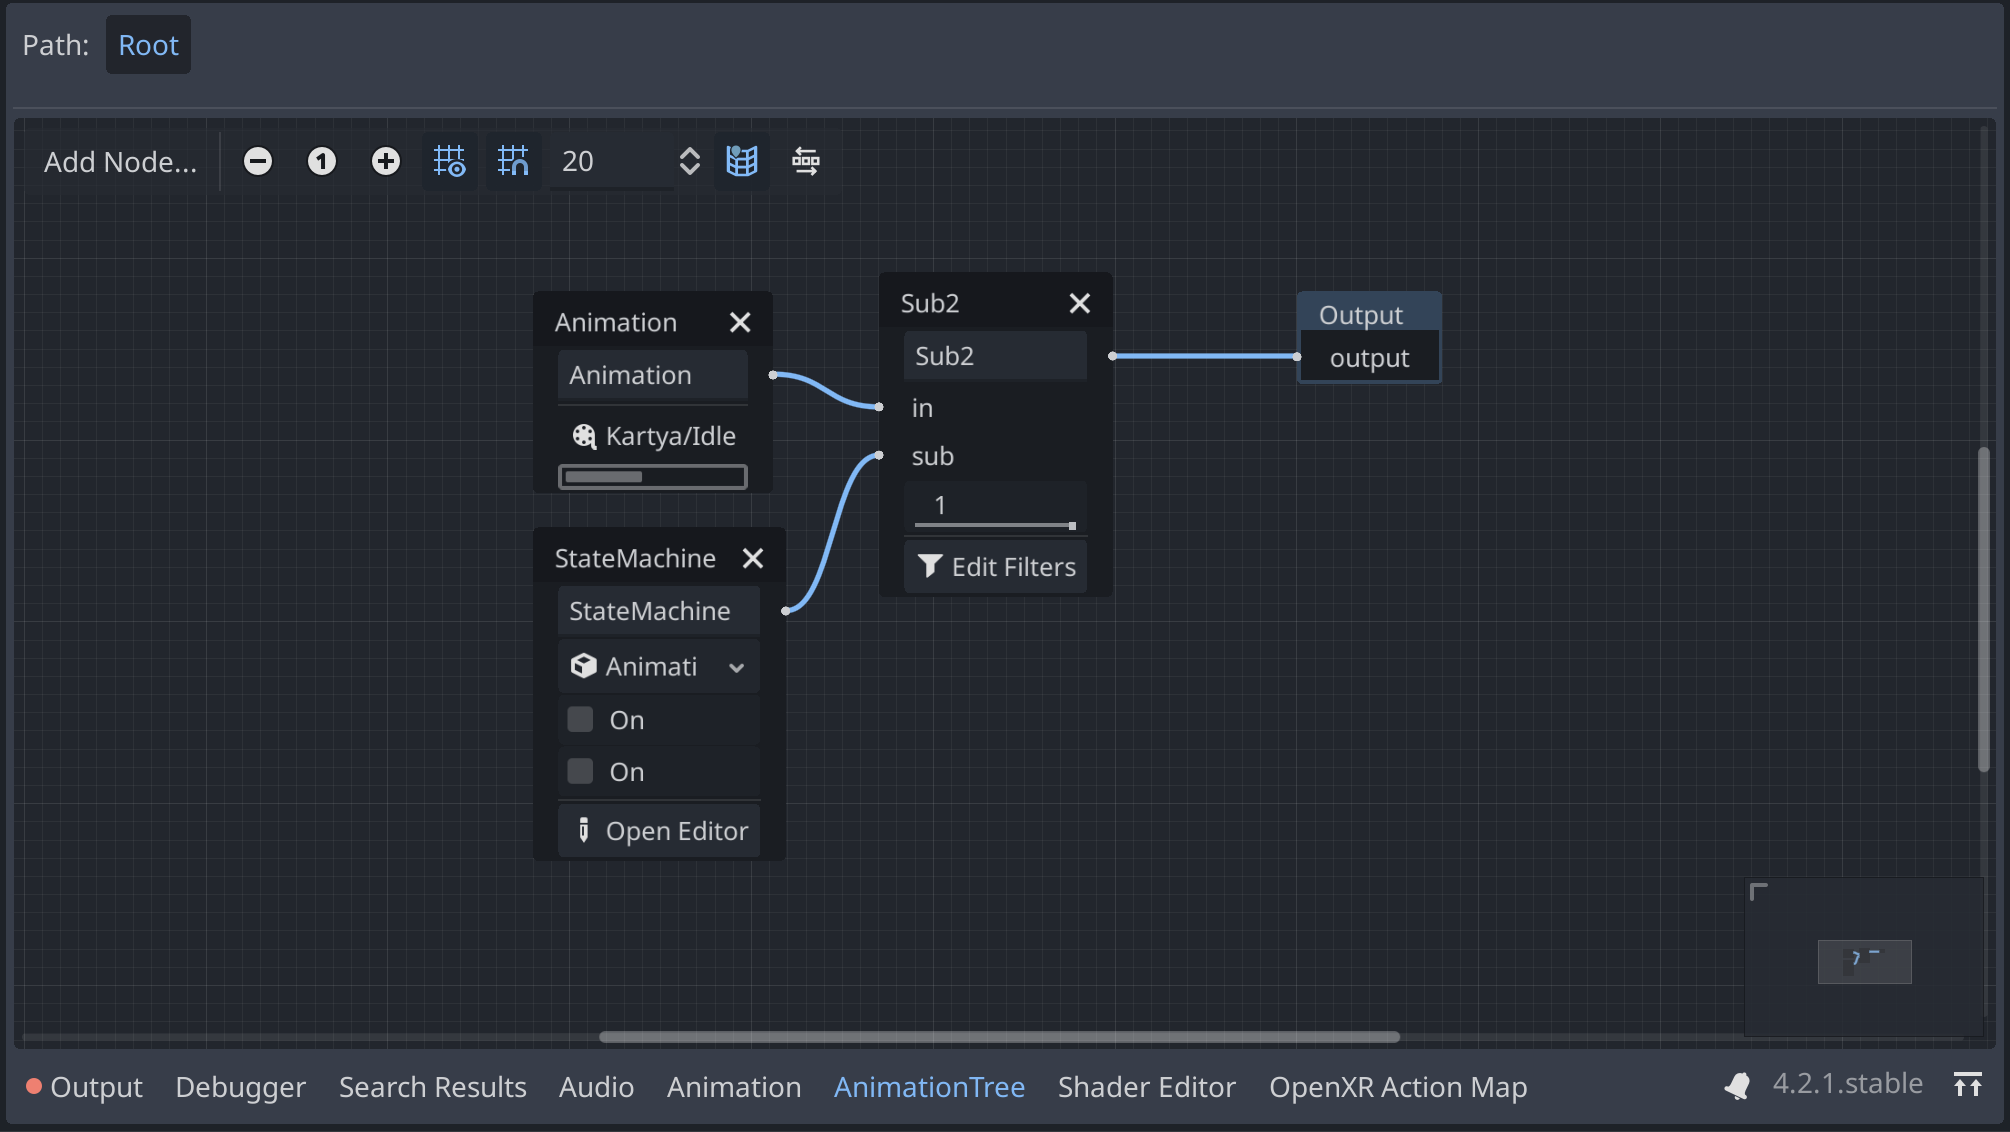
\includegraphics[width=\textwidth]{img/animation_tree.png}
    \caption{A Card animáció fája}
    \label{img:animation_tree}  
\end{figure}



